%
% riesz.tex -- 
%
% (c) 2019 Prof Dr Andreas Müller, Hochschule Rapperswil
%

%
% Lemma von Riesz
%
\section{Das Lemma von Riesz\label{section:riesz}}
%\rhead{Das Lemma von Riesz}
\index{Riesz!Lemma von}%
\index{Lemma von Riesz}%
Mit Hilfe der Partialbruchzerlegung war es im
Abschnitt~\ref{section:partialbruch}
möglich, die Funktion $M(\omega)$ als Polynom in $\cos\omega$ zu finden,
welches die Identität
\[
M(\omega) + M(\omega + \pi) = 1
\]
erfüllt.
Gesucht wird aber eine Funktion $H(\omega)$ mit
$M(\omega)=H(\omega)H(-\omega)$.
Bereits gefunden wurde ein $A(\omega)$ mit
$M(\omega)=(\cos^2\omega/2)^N A(\omega)$, gesucht wird jetzt noch 
eine Faktorisierung on $A(\omega)$ in $A(\omega)=B(\omega)B(-\omega)$.
Diese Faktorisierung wird ermöglicht dank des in diesem Abschnitt
formulierten und beschriebenen Lemmas von Riesz.
Das Lemma von Riesz ist die folgende, etwas überraschende Aussage:

\rhead{Das Lemma von Riesz}

\begin{lemma}[Riesz]
\label{lemma:riesz}
Ist
\[
A(\omega)
=
\sum_{k=0}^n
a_k \cos^k \omega,
\qquad
a_n\ne 0
\]
mit $A(0)=1$ und $A(\omega)\ge 0$ für alle $\omega$.
Dann gibt es eine Funktion
\[
B(\omega)
=
\sum_{k=0}^n b_ke^{-ik\omega}
\]
mit $B(0)=1$ und $A(\omega)=B(\omega)B(-\omega)$.
\end{lemma}

Der folgende Beweis verwendet die algebraischen Eigenschaften der
Nullstellen des trigonometrischen Polynoms $A(\omega)$.
Es ist daher immer wieder nötig, zwischen der Schreibweise mit
$\cos\omega$ und der komplexen Darstellung
\[
\cos\omega = \frac{e^{i\omega}+e^{-i\omega}}{2}
\]
hin- und her zu wechseln.
Dazu ist die rein algebraische Identität
\begin{align}
\frac{z+z^{-1}}2-\frac{s+s^{-1}}2
&=
\frac1{2s}(sz+sz^{-1}-s^2-1)
=
-
\frac1{2s}(1-sz-sz^{-1}+s^2)
\notag
\\
&=
-
\frac1{2s}(z-s)(z^{-1}-s)
\label{buch:kompakt:cosh}
\end{align}
nützlich, die im Folgenden wiederholt verwendet wird.
Man beachte, dass 
\[
\frac{s+s^{-1}}2
\ge 1\quad\text{für $s>0$}
\qquad\text{und}\qquad
\frac{s+s^{-1}}2
\le -1\quad\text{für $s<0$}
\]
gilt.

\begin{figure}
\centering
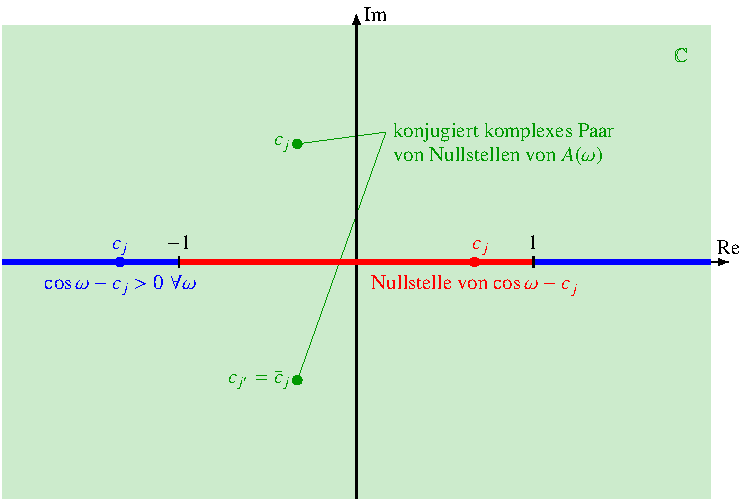
\includegraphics{chapters/8-kompakt/images/nullstellen.pdf}
\caption{Lokalisierung der Nullstellen von $A(\omega)$ in der komplexen
Ebene.
\label{kompakt:figure:nullstellen}}
\end{figure}

\begin{proof}[Beweis des Lemmas von Riesz]
Die Funktion $A(\omega)$ kann geschrieben werden als
$A(\omega) = p(\cos\omega)$, wobei $p(x)$ ein Polynom vom
Grad $n$ ist.
Das Polynom $p(x)$ hat $n$ möglicherweise komplexe Nullstellen
$c_1,\dots,c_n$, wobei komplexe Nullstellen in konjugiert komplexen
Paaren auftreten.
Das Polynom $p(x)$ kann daher faktorisiert werden in das Produkt
\begin{align*}
p(x)
&=
a_n(x-c_1)(x-c_2)\dots(x-c_n)
=
a_n \prod_{j=1}^n (x-c_j)
\\
A(\omega) = p(\cos\omega)
&=
a_n \prod_{j=1}^n (\cos \omega - c_j).
\end{align*}
Mit der Abkürzung $z=e^{-i\omega}$ können die Faktoren im Produkt als
\[
\cos\omega -c_j = \frac{z+z^{-1}}2-c_j
\]
geschrieben werden.

Wir versuchen, das gesuchte Polynom $B(\omega)$ aus Lösungen des Problems
für die einzelnen Faktoren von $p(x)$ aufzubauen.
Ein einzelner Faktor $A_j(\omega=)=\cos\omega - c_j$ erfüllt die Bedingungen an
$A$ im Lemma im Allgemeinen nicht.
Ist zum Beispiel $c_j$ reell zwischen $-1$ und $1$, dann hat
$\cos\omega-c_j$ eine Nullstelle und hat daher auch negative Werte.
Wenn $c_j$ komplex ist, dann ist $\cos\omega-c_j$ keine rellwertige
Funktion.
Es ist also notwendig, die Faktoren geeignet zu gruppieren,
was je nach Ort der Nullstelle in der komplexen Ebene auf andere
Weise zu geschehen hat (siehe auch Abbildung~\ref{kompakt:figure:nullstellen}).

Wir unterscheiden daher die folgenden drei Fälle, die in
Abbildung~\ref{kompakt:figure:nullstellen} in unterschiedlichen Farben
dargestellt sind:
\begin{enumerate}
\item
Fall $|c_j|\ge 1$ und $c_j\in\mathbb R$ ({\color{blue}Blau} in
Abbildung~\ref{kompakt:figure:nullstellen}):
In diesem Fall kann $c_j$ geschrieben werden als
\[
c_j = \frac{s+s^{-1}}2
\quad
\text{mit $s=\operatorname{sign}(c_j)\cdot \operatorname{arcosh}|c_j|$.}
\]
Dann wird
\[
A_j(\omega)
=
\cos\omega - c_j
=
\frac{z+z^{-1}}2 - \frac{s+s^{-1}}2
=
-\frac1{2s} (z-s)(z^{-1}-s)
\]
mit Hilfe von \eqref{buch:kompakt:cosh}.
Falls $c_j < 0$ ist auch $s<0$ und wir können dem Produkt $B(\omega)$
den Faktor $B_j(\omega)=(z-s)/\sqrt{-2s}$ hinzufügen, für den gilt
$B_j(\omega)B_j(-\omega)=A_j(\omega)$.
Falls $c_j > 0$ ist auch $s>0$ und wir können dem Produkt $B(\omega)$
den Faktor $B_j(\omega) =(z-s)/\sqrt{2s}$ hinzufügen, für den
gilt $B_j(\omega)B_j(-\omega)=-A_j(\omega)$.
Das Vorzeichen im zweiten Fall stört nicht, weil wegen $A(\omega)\ge 0$
noch ein weiterer Faktor $A_{j'}(\omega)$ vorhanden sein muss, der ebenfalls
$A_{j'}(\omega)\le 0$ ist für alle $\omega$ und der daher ebenfalls
mit dem ``falschen'' Vorzeichen in das Produkt eingeht, wodurch das
Vorzeichen wieder korrigiert wird.
\item
Fall $|c_j| < 1$ und $c_j\in\mathbb R$ ({\color{red}Rot} in
Abbildung~\ref{kompakt:figure:nullstellen}):
In diesem Fall hat $A_j(\omega)$ und damit $A(\omega)$ eine Nullstelle
für jedes $\omega$ mit $\cos\omega=c_j$.
Wegen $A(\omega)\ge 0$ müssen alle solchen Nullstellen in gerader
Anzahl auftreten.
Sei $\alpha$ so, dass $\cos\alpha = c_j$ und damit insbesondere auch
\[
c_j
=
\cos\alpha
=
\frac{s+s^{-1}}2
\quad\text{mit $s=e^{i\alpha}$}.
\]
Wegen der Symmetrie der Funktion $\cos\omega$ gilt auch
\[
c_{j'}=
\cos(-\alpha)
=
\frac{e^{-i\alpha}+e^{i\alpha}}2.
\]
Damit kann $A_j(\omega)^2$ geschrieben werden als
\begin{align*}
A_j(\omega)^2
&=
\biggl(
\frac{z+z^{-1}}2-\frac{e^{i\alpha}+e^{-i\alpha}}2
\biggr)
\,
\biggl(
\frac{z+z^{-1}}2-\frac{e^{-i\alpha}+e^{i\alpha}}2
\biggr)
\\
&=
\frac{1}{2e^{i\alpha}}
(z-e^{i\alpha})
(z^{-1}-e^{i\alpha})
\frac{1}{2e^{-i\alpha}}
(z-e^{-i\alpha})
(z^{-1}-e^{-i\alpha})
\\
&=
\frac{1}{2}
(z-e^{i\alpha})
(z-e^{-i\alpha})
\cdot
\frac{1}{2}
(z^{-1}-e^{i\alpha})
(z^{-1}-e^{-i\alpha})
\\
&=
\frac{1}{2}
(z^2-2z\cos\alpha +1)
\cdot
\frac{1}{2}
(z^{-2}-2z^{-1}\cos\alpha +1).
\end{align*}
Wir fügen daher der Funktion $B(\omega)$ den Faktor
$B_j(\omega)=\frac12(z^2-2z\cos\alpha +1)$ hinzu, für
den 
$B_j(\omega)B_j(-\omega)=A_j(\omega)^2$ gilt.
\item
Fall $c_j\in\mathbb C\setminus\mathbb R$ ({\color{darkgreen}Grün} in
Abbildung~\ref{kompakt:figure:nullstellen}):
In diesem Fall gibt es eine zweite, komplex konjugierte Nullstelle mit
$c_{j'}=\bar{c}_j$.
Wir möchten $c_j$ wieder als
\begin{equation}
c_j
=
\frac{s+s^{-1}}2
\label{buch:kompakt:cj}
\end{equation}
darstellen.
Dazu multiplizieren wir \eqref{buch:kompakt:cj} mit $s$ und erhalten die
quadratische Gleichung
\[
s^2-2c_j s+1=0
\]
mit der Lösung
\[
s=c_j\pm\sqrt{c_j^2-1},
\]
die immer mindestens eine Lösung hat.
Wir dürfen daher annehmen, dass
\[
c_j = \frac{s+s^{-1}}2
\qquad\text{und}\qquad
c_{j'} = \bar{c}_j = \frac{\bar{s}+\bar{s}^{-1}}2.
\]
Damit können wir jetzt das Produkt $A_j(\omega)A_{j'}(\omega)$ 
wie folgt faktorisieren:
\begin{align*}
A_j(\omega)A_{j'}(\omega)
&=
\biggl(
\frac{z+z^{-1}}2 - \frac{s+s^{-1}}2
\biggr)
\,
\biggl(
\frac{z+z^{-1}}2 - \frac{\bar{s}+\bar{s}^{-1}}2
\biggr)
\\
&=
\frac{1}{2s}
(z-s)(z^{-1}-s)
\cdot
\frac{1}{2\bar{s}}
(z-\bar{s})(z^{-1}-\bar{s})
\\
&=
\frac{1}{4|s|^2}(z-s)(z^{-1}-s)(z-\bar{s})(z^{-1}-\bar{s})
\\
&=
\frac1{2|s|}
(z-s)
(z-\bar{s})
\cdot
\frac1{2|s|}
(z^{-1}-s)
(z^{-1}-\bar{s})
\\
&=
\frac1{2|s|}(z^2-2z\operatorname{Re}s -|s|^2)
\cdot
\frac1{2|s|}(z^{-2}-2z^{-1}\operatorname{Re}s -|s|^2).
\end{align*}
Wir fügen in diesem Fall der Funktion $B(\omega)$ den Faktor
$B_j(\omega)=(z^2-2z\operatorname{Re}s-|s|^2)/2|s|$ hinzu.
\end{enumerate}
In allen drei Fällen haben wir für die behandelten Faktoren $A_j(\omega)$
und der eventuell zugehörigen Faktoren $A_{j'}(\omega)$ eine Funktion
$B_j(\omega)$ gefunden, so dass das Produkt all dieser Faktoren
\[
B(\omega)
=
\prod_j B_j(\omega)
\]
genau die im Lemma versprochenen Eigenschaften hat.
\end{proof}

Aus dem Beweis des Lemmas lässt sich auch ein Algorithmus ablesen, mit
dem das Polynom $B(\omega)$ konstruiert werden kann.
\begin{enumerate}
\item
Bestimme die Nullstellen von $A(\omega) = P((1-\cos \omega)/2)$ 
als Polynom in $\omega$ und schreibe $A(\omega)$ als Produkt
\[
A(\omega)
=
\prod_j A_j(\omega)
=
\prod_j (\cos\omega - c_j).
\]
\item Für jede Nullstelle $c_j$ mit $|c_j|>1$ füge einen Faktor 
\[
B_j(z)=\frac{1}{\sqrt{-2s}}(z-s),\qquad s = \operatorname{sign}c_j\cdot \operatorname{arcosh}|c_j|
\]
zu $B(z)$ hinzu (Fall {\color{blue}blau}).
\item
Jede Nullstelle $c_j \in\mathbb R$ mit $|c_j|<1$ kommt eine gerade Anzahl mal
vor.
Füge für jedes Paar von Nullstellen einen Faktor
\[
B_j(z) = \frac12(z^2 -2 z\cos \alpha +1),
\qquad\text{mit $c_j=\cos\alpha$}
\]
hinzu (Fall {\color{red}rot}).
\item
Für jede Nullstelle $c_j\in \mathbb C\setminus\mathbb R$ gibt es
eine konjugiert komplexe Nullstelle $c_{j'}=\bar{c}_j$.
Füge für beide einen Faktor
\[
B_j(z) = \frac{1}{2|s|}(z^2 -2z\operatorname{Re}s-|s|^2),
\qquad
\text{wobei $s$ eine Lösung von $s^2 -2c_js+1=0$ ist,}
\]
hinzu (Fall {\color{darkgreen}grün}).
\end{enumerate}

\begin{beispiel}
\label{buch:kompakt:db2riesz}
Als Beispiel für den im Beweis des Lemmas von Riesz formulierten Algorithmus
wenden wir ihn auf das Polynom
\[
A(\omega)
=
2-\cos\omega
=
2-\frac12(e^{i\omega}+e^{-i\omega})
\]
an, welches wir für den Fall $N=2$ im nächsten Abschnitt brauchen werden.

Das Polynom $-(\cos\omega -2)$ hat nur einen einzigen Faktor mit $c_0=2$,
dies entspricht dem Fall {\color{blue}blau} in
Abbildung~\ref{kompakt:figure:nullstellen}.
Der Faktor $B_j(z)$ muss daher von der Form $B_j(z)=b_0+b_1z$ sein.
Setze man dies für $B_j$ ein, erhält man
\[
A(\omega)
=
2-\cos\omega
=
(b_0+b_1e^{i\omega})
(b_0+b_1e^{-i\omega})
=
b_0^2 + b_1^2 +b_0b_1\cos\alpha 
\]
Durch Koeffizientengleich liest man ab
\begin{align*}
2&=b_0^2 + b_1^2
\\
-\frac12&=b_0b_1.
\end{align*}
Setzt man die zweite Gleichung in die erste ein, erhält man die biquadratische
Gleichung
\[
2=b_0^2 + \frac{1}{4b_0^2}
\qquad\Leftrightarrow\qquad
b_0^4-2b_0^2 + \frac14 = 0
\]
mit den Lösungen
\[
b_0^2 = 1\pm \sqrt{1-\frac14} = \frac{2\pm\sqrt{3}}{2}
\qquad\Rightarrow\qquad
b_0 = \pm \frac{1\pm\sqrt{3}}2.
\]
Tatsächlich ist
\[
\biggl(
\frac{1\pm\sqrt{3}}2
\biggr)^2
=
\frac{1\pm 2\sqrt{3}+3}{4}
=
\frac{2\pm\sqrt{3}}2.
\]
Die zugehörigen Werte von $b_1$ sind
\[
b_1
=
\mp
\frac{1}{2}\frac{2}{1\pm\sqrt{3}}
=
\mp
\frac{1}{1\pm\sqrt{3}}
=
\mp
\frac{1\mp \sqrt{3}}{1-3}
=
\pm
\frac{1\mp\sqrt{3}}{2}.
\]
Wählt man in allen Fällen das obere Zeichen, wird
\[
B(\omega)
= 
\frac{1+\sqrt{3}}2 + \frac{1-\sqrt{3}}2 e^{i\omega}.
\]
\end{beispiel}


